\section{Results}

\begin{figure*}
    \centering
    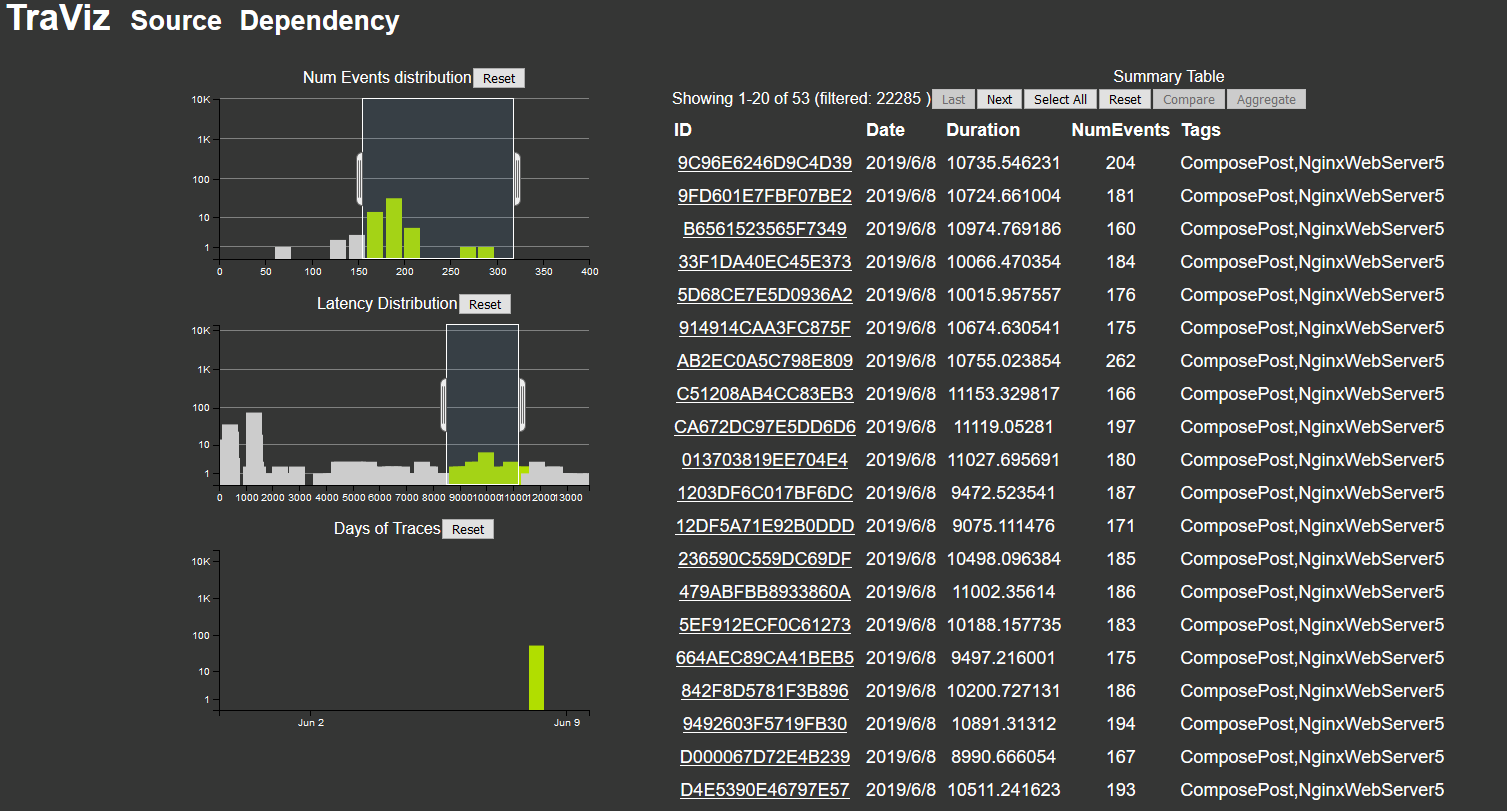
\includegraphics[width=\textwidth]{fig/outlier}
    \caption{Example of filtering along the Num Events and Duration dimension to look at one specific set of outliers}
    \label{fig:outlier}
\end{figure*}

\subsection{Use Case 1: Outlier detection}

The user has received multiple bug reports from different customers
about some requests taking tens of seconds to complete when they
usually take fewer than a second to complete. To investigate, the
user opens up TraViz and sees the distribution of the traces. The
user can quickly see that there are a small number of traces
that have indeed taken unusually long as compared to other traces.
The user selects a specific duration range to filter so that
they can only see the list of traces that have their duration
within that range. To further narrow down, the user selects
an events range to further reduce the number of traces as shown
in Figure ~\ref{fig:outlier}. The user can now start performing
root cause analysis.

\begin{figure*}
    \centering
    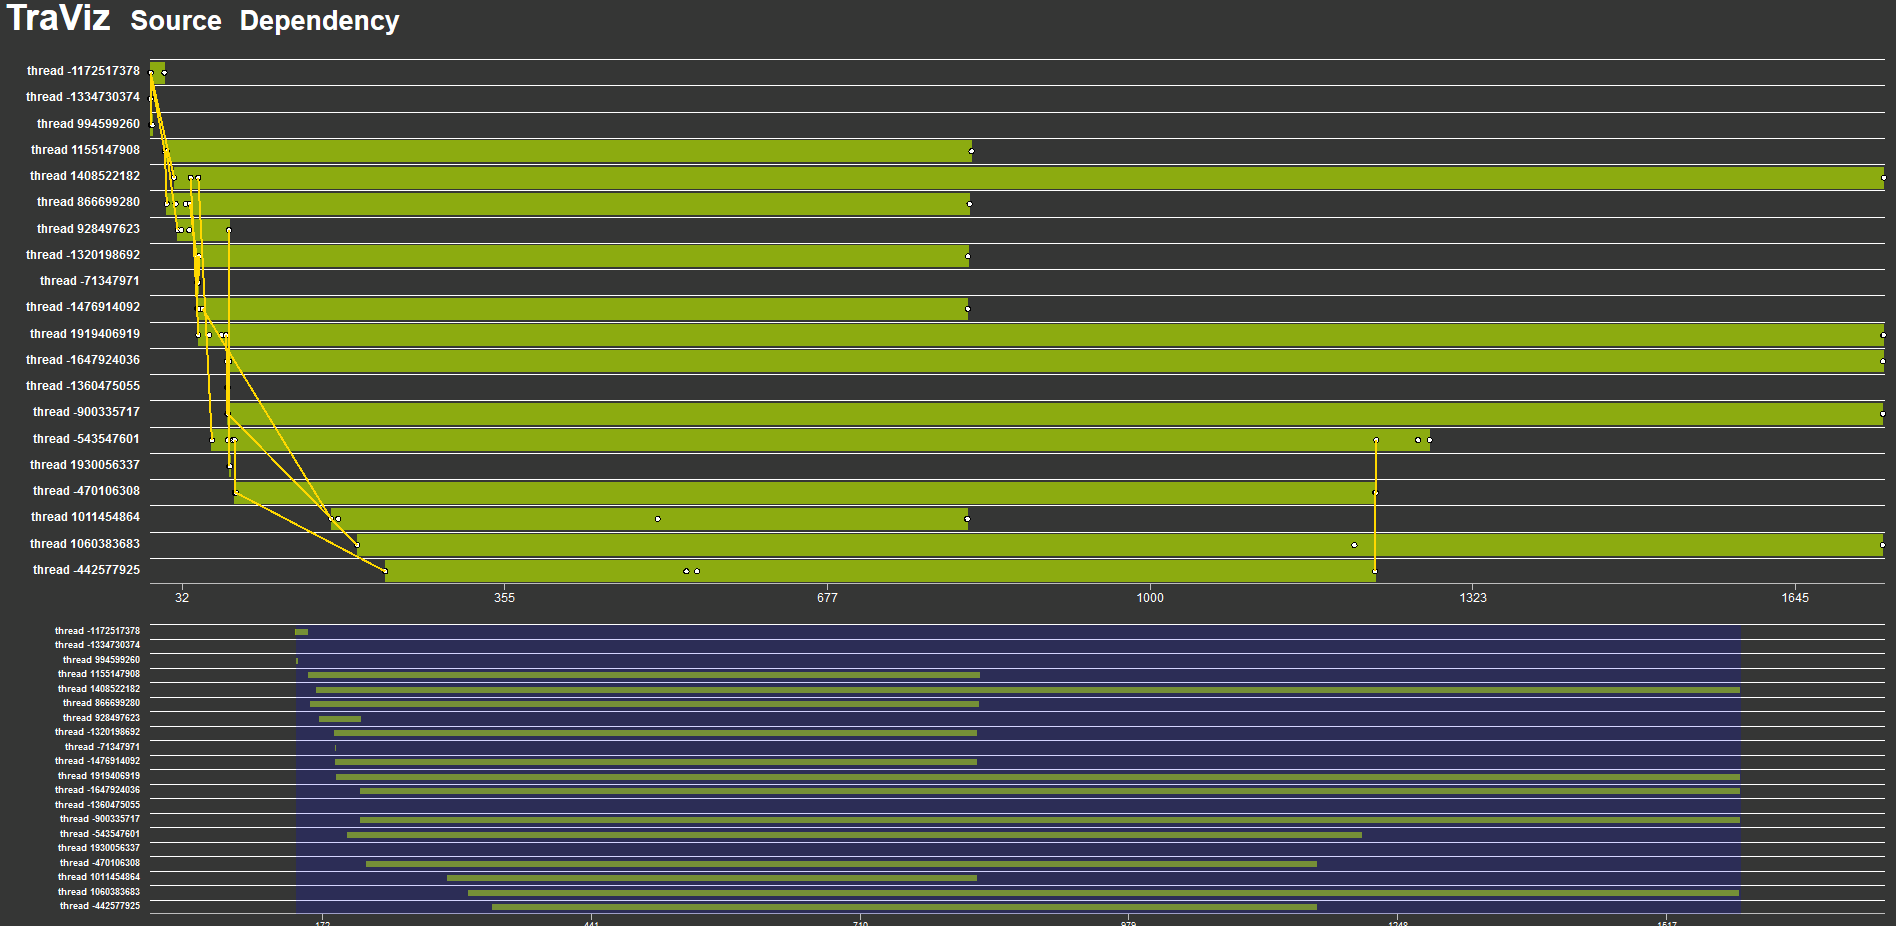
\includegraphics[width=\textwidth]{fig/swimlane}
    \caption{Swimlane view of trace ID AB2EC0A5C798E809 from the DeathStarBench dataset}
    \label{fig:outlier}
\end{figure*}

\subsection{Use Case 2: Performance Analysis on a single trace}

Now that the user has a picked a filtered set of traces, the user
can take a look at an individual trace to figure out the root
cause of the performance issue. The user clicks on one of the
traces from the filtered list to see the detailed view
of the trace ~\ref{fig:swimlane}. From a cursory look,
the user can identify which thread takes the longest time to complete
its execution and correctly identify the set of events that caused delay
on the trace.

\subsection{Use Case 3: Finding differences in pair of traces}

\subsection{Use Case 4: Finding similarities in groups of traces}

\subsection{Use Case 5: Source Code Optimization}

\begin{figure*}
    \centering
    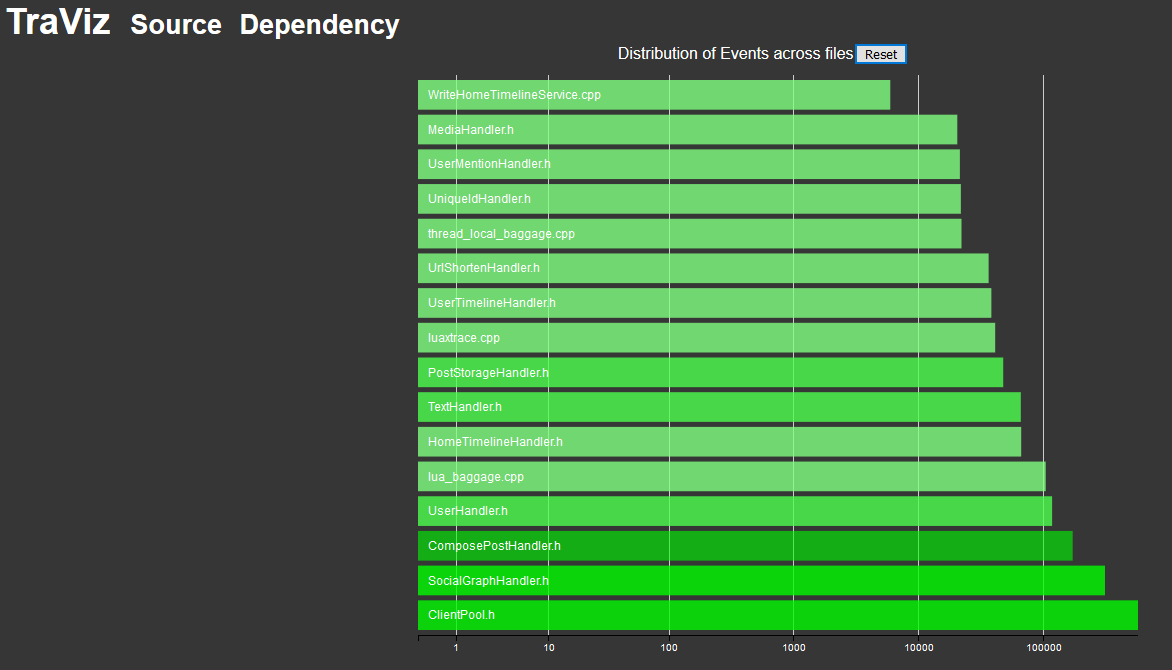
\includegraphics[width=\textwidth]{fig/sourcecode1}
    \caption{The distribution of the events across the files for the DeathStarBench dataset, with colour showing the number of lines from the
    file that produced these events.}
    \label{fig:source1}
\end{figure*}

\begin{figure*}
    \centering
        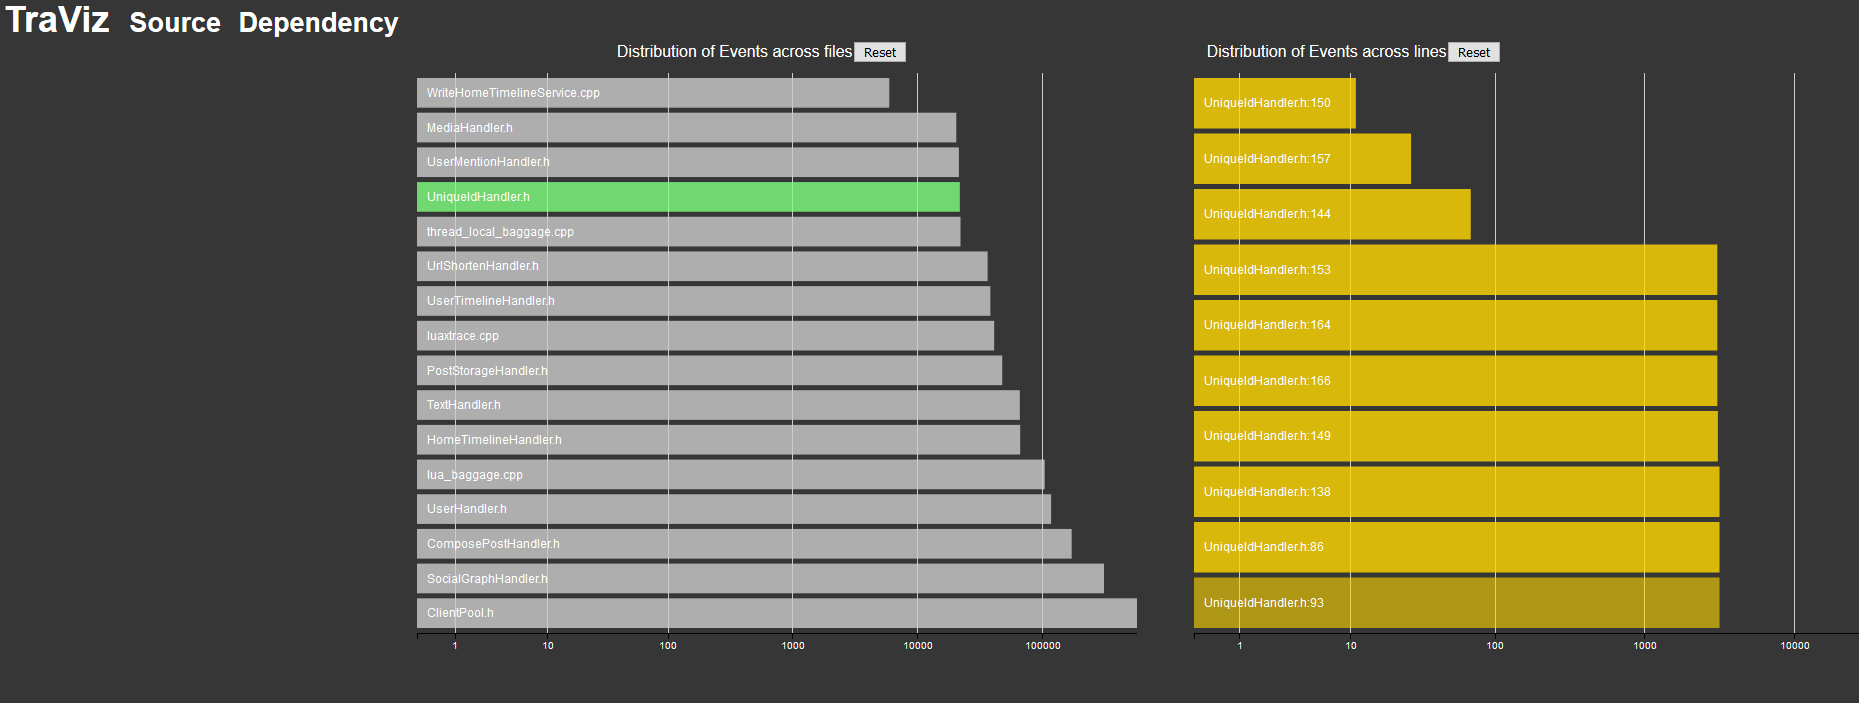
\includegraphics[width=\textwidth]{fig/sourcecode2}
        \caption{The distribution of events across the lines for the UniqueIdHandler file}
        \label{fig:source2}
\end{figure*}

The user wants to know what files in the source code, Specifically
what lines in the source code are producing the most number of events
in traces as well as producing the least number of events in traces.
The user clicks on the Source tab on the navigation bar
to land at the source page to see the distribution of events
across files in sorted order as shown in Figure ~\ref{fig:source1}.
To view the distribution of events across the lines in a particular
file, the user clicks on the bar with the name of the target file.
This gives rise to another chart which shows the distribution
of the events across lines in that file in sorted order as shown
in Figure ~\ref{fig:source2}. To view the line in the context of the source
code, the user clicks on the bar of that specific line to get
redirected to that specific line in the specific file on github.

\subsection{Use Case 6: Service Dependency Analysis}

\begin{figure*}
    \centering
    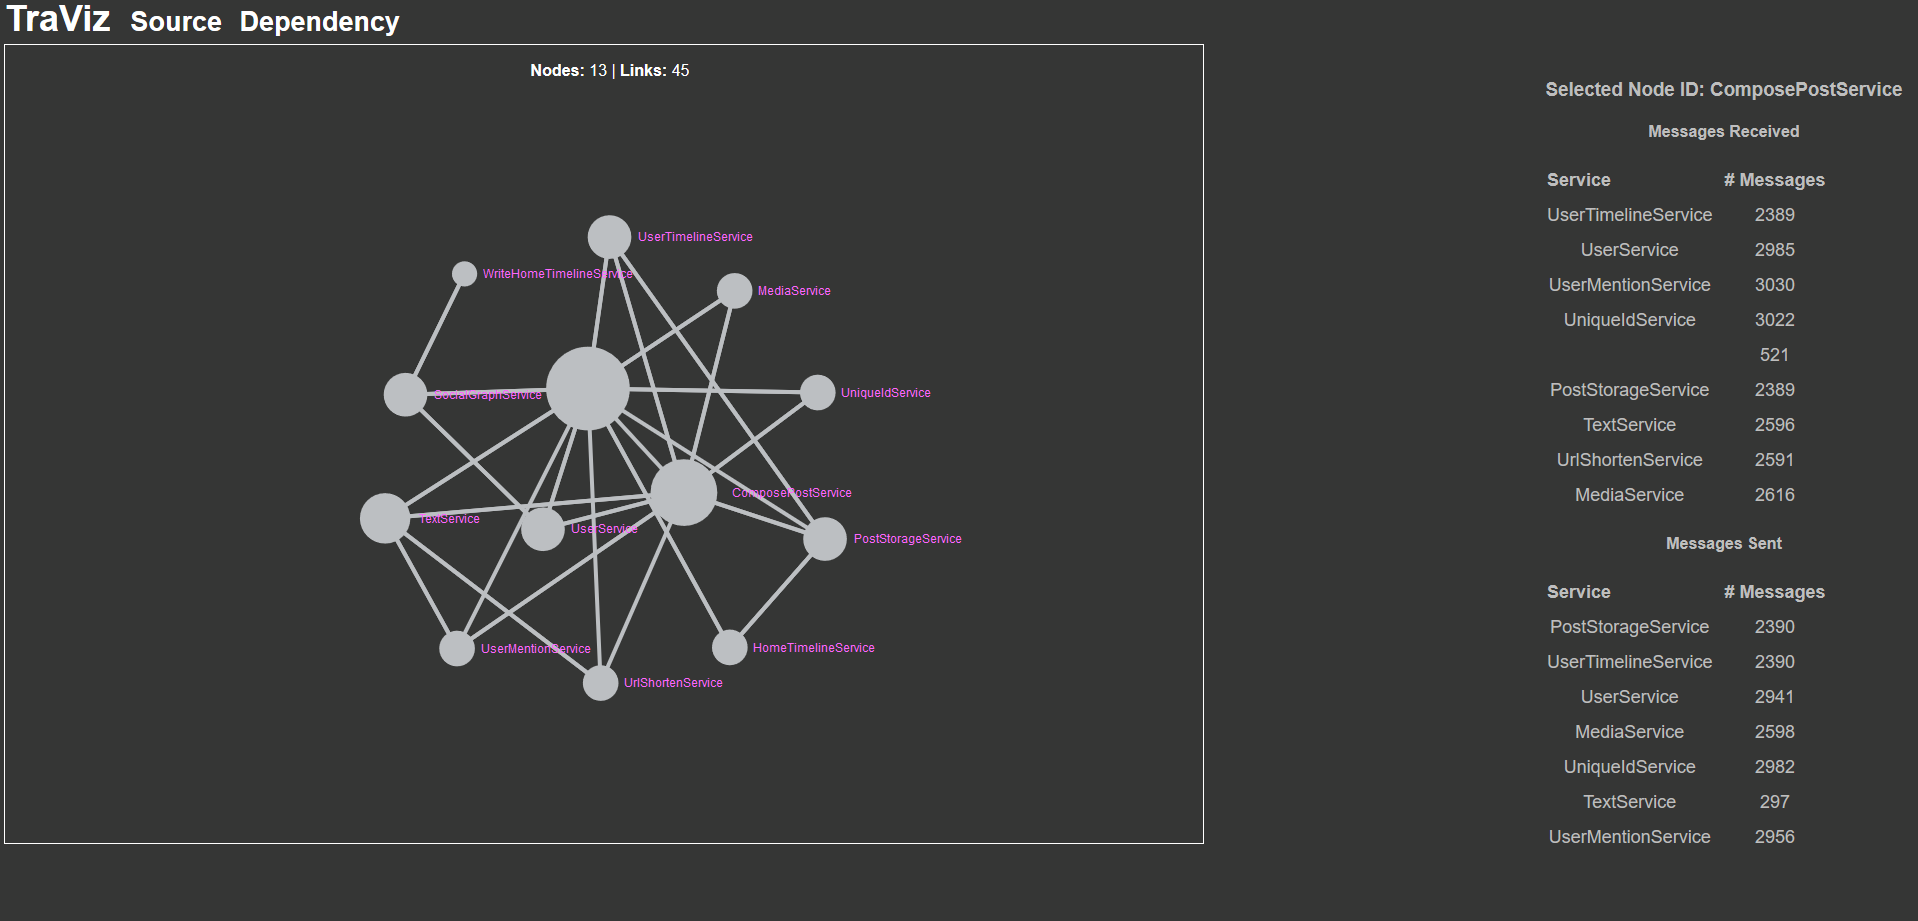
\includegraphics[width=\textwidth]{fig/dependency}
    \caption{The dependency graph shows how the services in the system interact with each other. 
    The detail view shows the messages received and sent by the nodes running that specific service from
    the nodes running other services. This figure shows the breakdown for the ComposePostService from the DeathStar
    Microbenchmark suite.}
    \label{fig:dependency}
\end{figure*}

The user wants to know how the different services in the distributed
system interacts with each other. Specifically, the user wishes to know
the load each service is receiving from all the other services in the system.
To accomplish this, the user clicks on the Dependency tab on the navigation bar
to land at the dependency page to see the dependency graph as shown in Figure ~\ref{fig:dependency}.
To find out detailed information about each service, the user clicks on the node with
the particular service to bring up the detailed view of the service which shows
the number of messages received by that service from every other service, and the number
of messages sent by that service to every other service.

\subsection{Informal User Study}

To evaluate the efficacy of TraViz, we conducted a very Informal user study
with 2 target users. One of the target users is one of the leading experts in distributed
tracing whereas the other user is an engineer at a large internet company where part of
their job is to analyze distributed traces. Due to geographical and time constraints,
the user study had to be done asynchronously where the target users were given
a deployed link of our tool and were asked to provide feedback regarding the user
experience.

Both of the target users liked the overview dashboard. Specifically, the leading expert
stated "Incorporating high-level metrics side-by-side with trace search and selection is a good idea and I like the dashboard you came 
up with". The source code view also garnered positive reviews as both the users thought
this is something that they would like to use with their data. The source code view
piqued the interest of the expert user as they thought it had the potential of getting
very deep as it was combining the static source code of the system with dynamic information
about actual executions. The other user thought the most useful visualization was the individual
trace view as it allowed them to view time spent by each thread individually.
The expert user thought that the dependency graph was useful but commented that
the graph should be directed as that is what users expect to see.

For the trace comparison and aggregation idioms, there was a general sense of confusion
across both the users. One of the users was particularly confused as to what each
of the nodes meant in the graph - whether the nodes were showing performance information
or structural differences or both. The expert user commented that the comparison and aggregation
graphs have some underlying ordering which wasn't being visualized. Although, they did acknowledge
that getting the ordering right for comparisons and aggregations is a hard task.

Given the feedback from the users, we believe that TraViz is partially successful in its endeavor of
being the most usable distributed tracing visual analysis tool.